% !TEX program = xelatex
\documentclass[12pt]{report}
\usepackage{unicode-math}
\usepackage{amsmath}
\usepackage{amsthm}
\usepackage{xltxtra}
\usepackage{appendix}


\usepackage{polyglossia}
\setmainlanguage{bulgarian}
\setotherlanguage{english}


\defaultfontfeatures{Ligatures=TeX}
\setmainfont{Comfortaa-Regular}
%setmathfont{Neo Euler}
\newfontfamily\cyrillicfont{Comfortaa-Regular}

% \usepackage[english, bulgarian]{babel}
% \usepackage{indentfirst}
\usepackage[a4paper, portrait, margin = 1.5 cm]{geometry}
\usepackage{url}
\usepackage{color}
\usepackage{float}
\usepackage{xcolor}
\usepackage{graphicx}
\usepackage{listings}
\usepackage{subfig}
\usepackage[export]{adjustbox}
\usepackage{blindtext}
\usepackage{scrextend}
\usepackage{amsfonts}
\usepackage[parfill]{parskip}
\usepackage{multicol}
\usepackage{mathtools}
\usepackage{pgfplots}

\newtheorem{theorem}{Пример}
\newtheorem*{definition*}{Дефиниция}

\numberwithin{equation}{section}
\numberwithin{figure}{section}
\addtokomafont{labelinglabel}{\sffamily}

\def\changemargin#1#2{\list{}{\rightmargin#2\leftmargin#1}\item[]}
\let\endchangemargin=\endlist 
\renewcommand{\baselinestretch}{1.1}
\setlength{\emergencystretch}{3em}

\usepackage{graphicx}
\graphicspath{ {./resources/} }

\lstset{
	backgroundcolor = \color{light-gray},
    language = C,
    xleftmargin = 1cm,
    framexleftmargin = 1em,
    basicstyle=\ttfamily,
	moredelim=[is][\underbar]{_}{_},
}


\usepackage{color}
\definecolor{Bluish}{rgb}{0.39,0.55,0.78}
\definecolor{light-gray}{gray}{0.9}

\usepackage{hyperref}
\hypersetup{
    colorlinks=true,
    linktoc=all,
    citecolor=black,
    filecolor=black,
    linkcolor=black,
    urlcolor=black
}
\makeatletter
\ifdefined\HyLang@bulgarian\else
\appto\blockextras@bulgarian{%
  \def\equationautorefname{\text{Уравнение}}%
  \def\footnoteautorefname{\text{Бележка}}%
  \def\itemautorefname{item}%
  \def\figureautorefname{\text{Фигура}}%
  \def\tableautorefname{\text{Таблица}}%
  \def\partautorefname{Part}%
  \def\appendixautorefname{Appendix}%
  \def\chapterautorefname{chapter}%
  \def\sectionautorefname{section}%
  \def\subsectionautorefname{subsection}%
  \def\subsubsectionautorefname{subsubsection}%
  \def\paragraphautorefname{paragraph}%
  \def\subparagraphautorefname{subparagraph}%
  \def\FancyVerbLineautorefname{line}%
  \def\theoremautorefname{\text{Пример}}%
  \def\pageautorefname{page}%
}
% \inlineextras@bulgarian is empty, so we simply set it
% equal to \blockextras@bulgarian
\let\inlineextras@bulgarian\blockextras@bulgarian
\fi
\makeatother

\usepackage{tabularx}

\newcommand{\B}[1]{\left(#1\right)}
\newcommand{\Q}[1]{\left[#1\right]}


\title{Дипломна работа}
\author{Диана Генева <dageneva@qtrp.org>}
\date{2018}

\begin{document}
\maketitle
\thispagestyle{empty}
\tableofcontents
\pagebreak

\chapter{Нулева зона}
Бла, бла, бла, аз съм толкова емоционална. 
Не знам


\includegraphics[width=0.5\textwidth ]{pikachu}
\chapter{Емоции в реч}
\label{chap:speech}

    \section{Физика на тъгата}
    Вокален тракт е общото название на кухините над ларингса (гръкляна), през които минава въздуха при генериране на реч.
    При хората той се състои от ларингеална кухина, фарингс, устна кухина и носна кухина, които могат да се видят на Фиг. 1.
    Вокалният тракт е отговорен за произвеждане на различни звуци, като текущата конфигурация на отделните му компоненти определя самия звук.
    Според [https://ieeexplore.ieee.org/document/4809202], освен конкретния звук, конфигурацията на вокалния тракт зависи и от емоцията, която изпитва говорещият. 
    Из българската литература се срещат изречения като "страхът стискаше гърлото, задушаваше гласа"[Гласовете ви чувам] и изрази като "буца в гърлото" или "пресъхнало гърло" са станали синоними за дадено емоционално
    състояние в разговорната реч. Тези фрази имат физиологично обяснение и влияят върху характеристиките на произведената реч.
    Именно затова бихме искали да можем математически да моделираме конфигурацията на вокалния тракт и да извличаме характеристики от нея.
    \begin{figure}[ht]%
        \centering
        \begin{changemargin}{0cm}{0cm} 
            \subfloat[Физическо представяне на вокалния тракт]{%
                \label{fig:physics:1:a}

                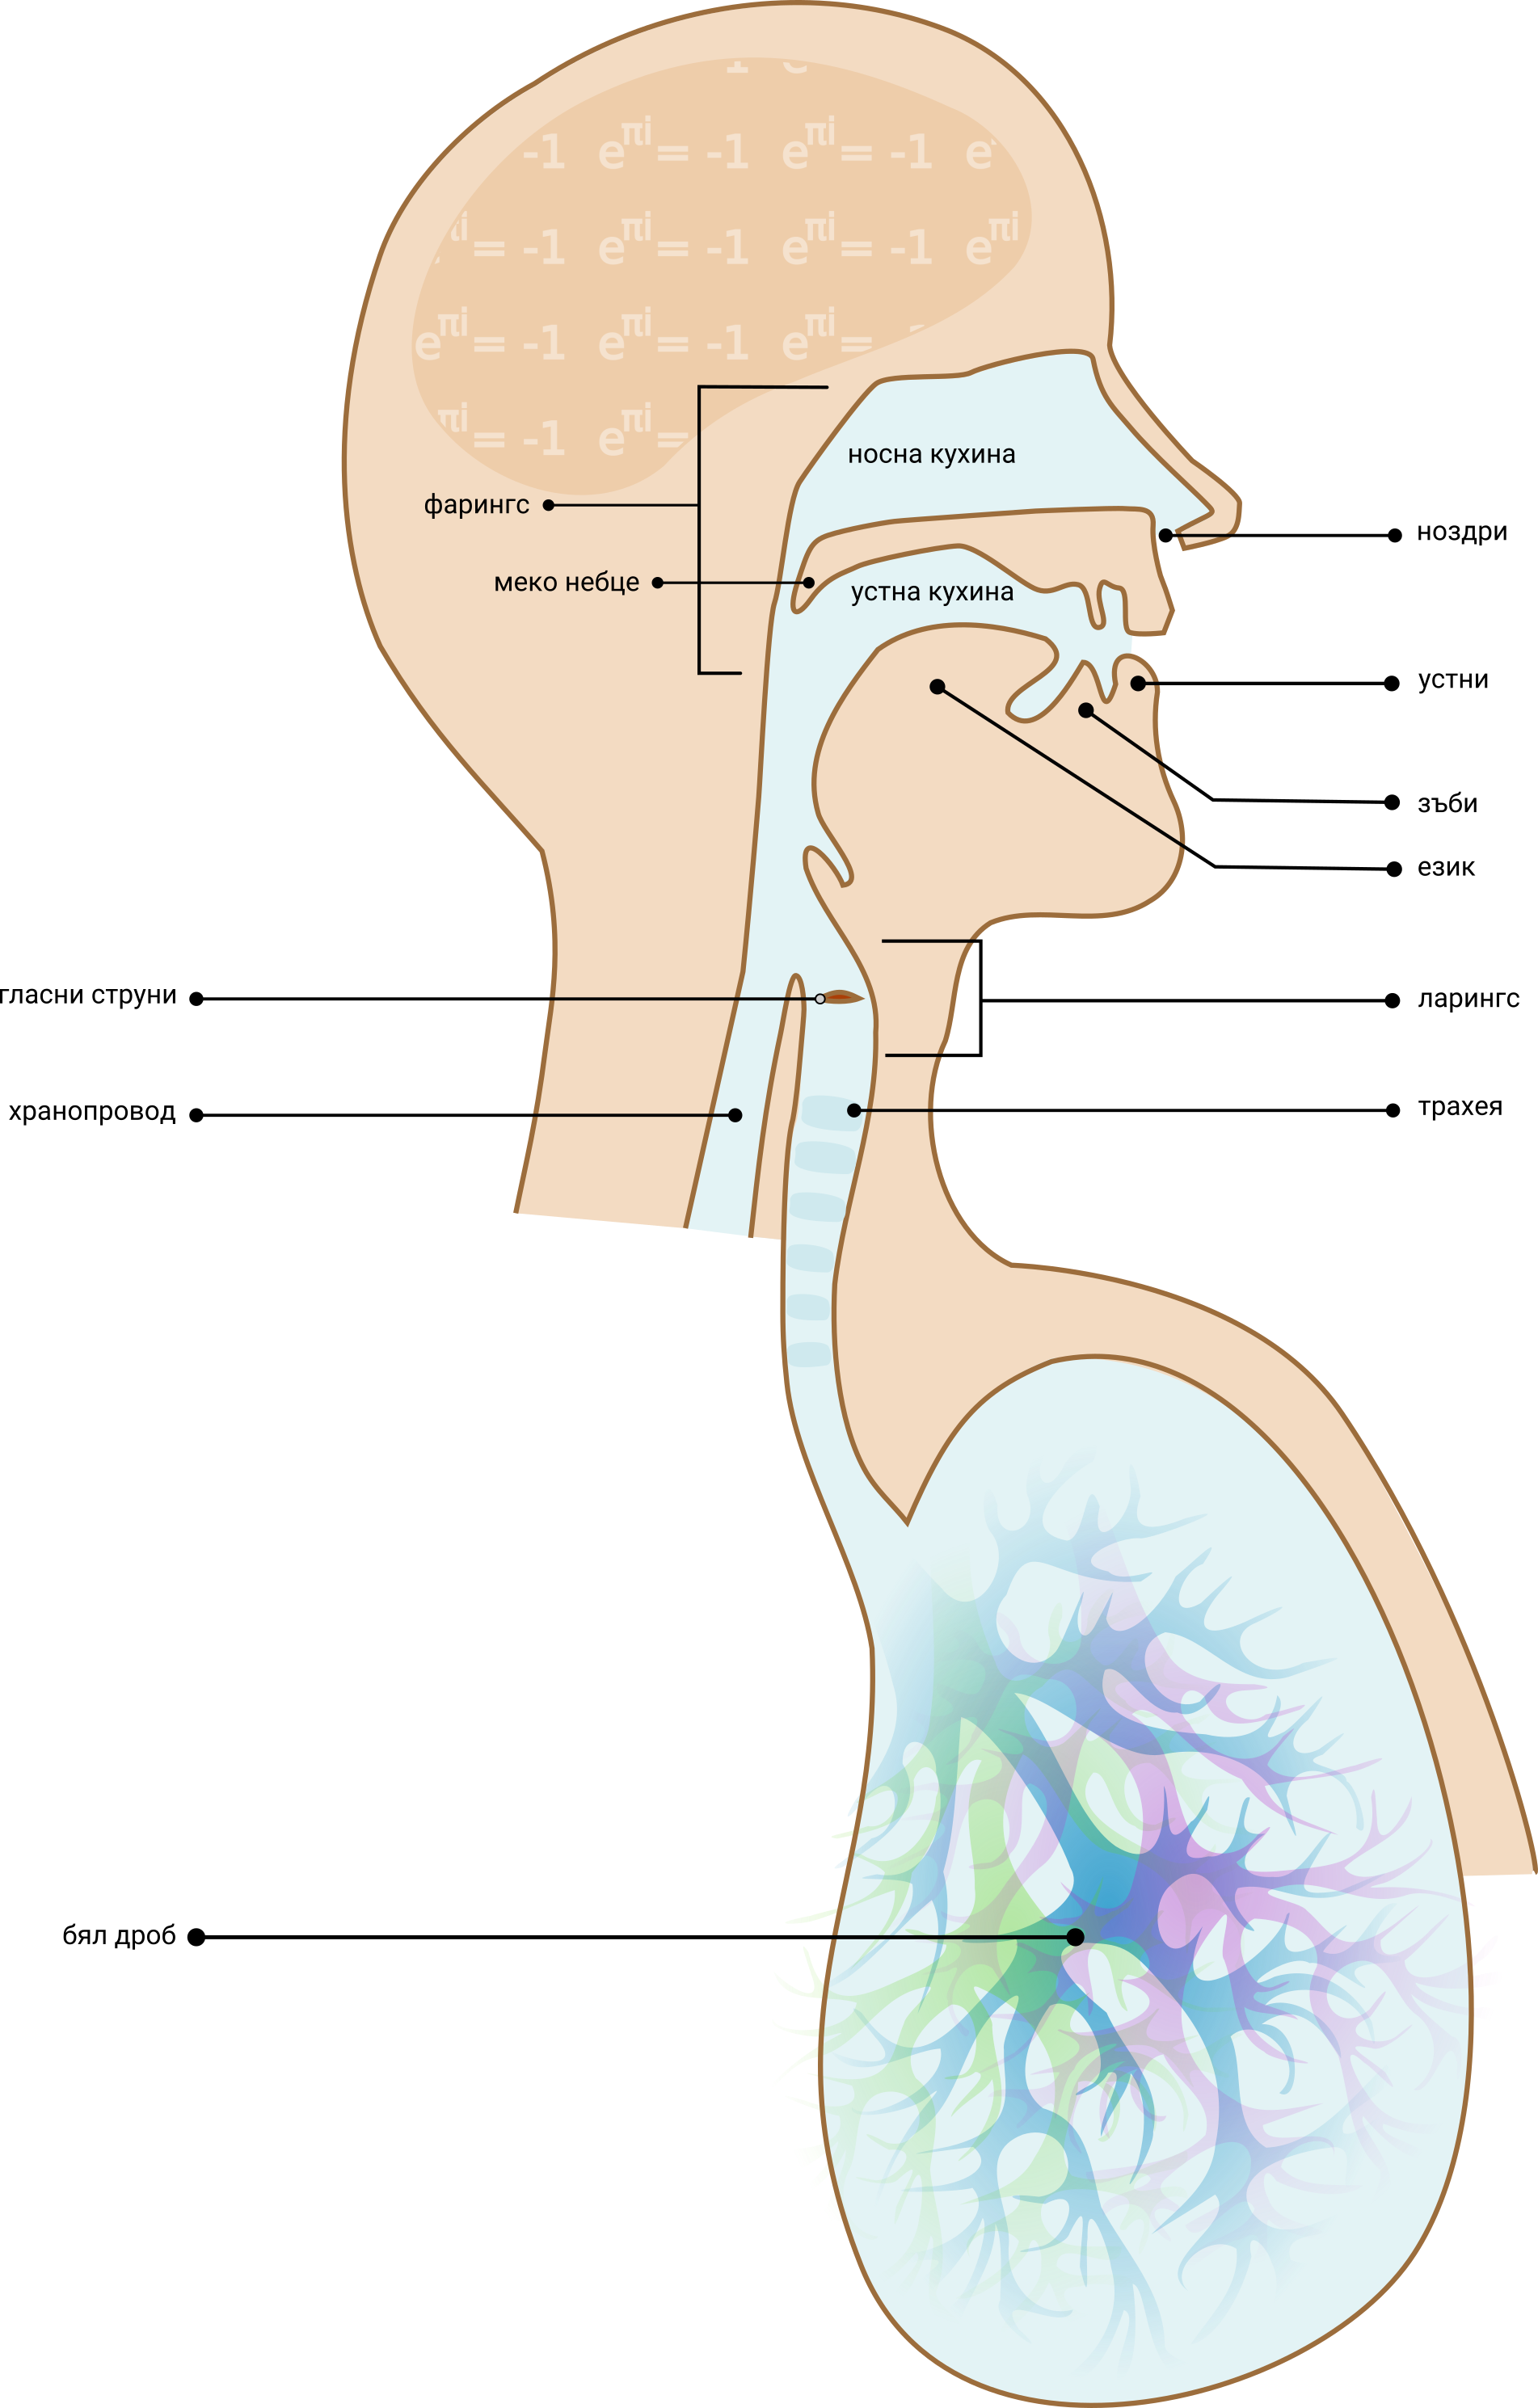
\includegraphics[width=0.48\paperwidth,valign=t]{physics}%
            } \hspace{0.8cm}
            \subfloat[Опростено представяне на вокалния тракт]{%
                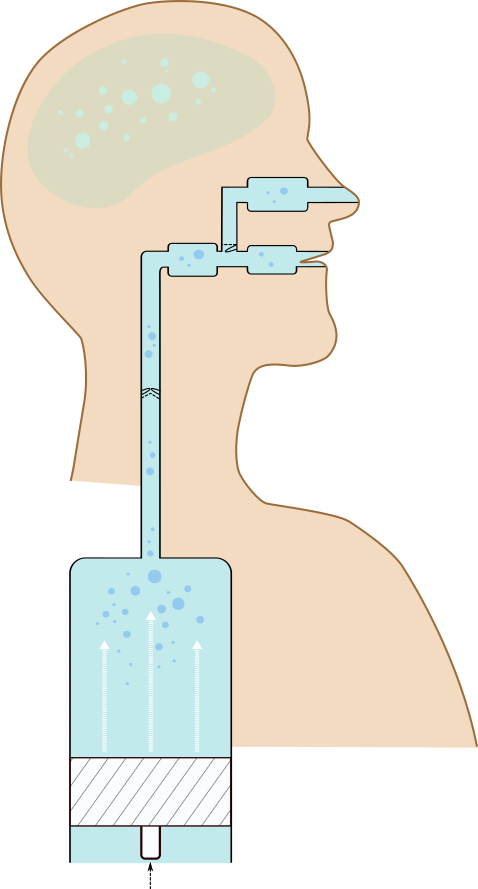
\includegraphics[width=0.28\paperwidth,valign=t]{tubes}%
                \vphantom{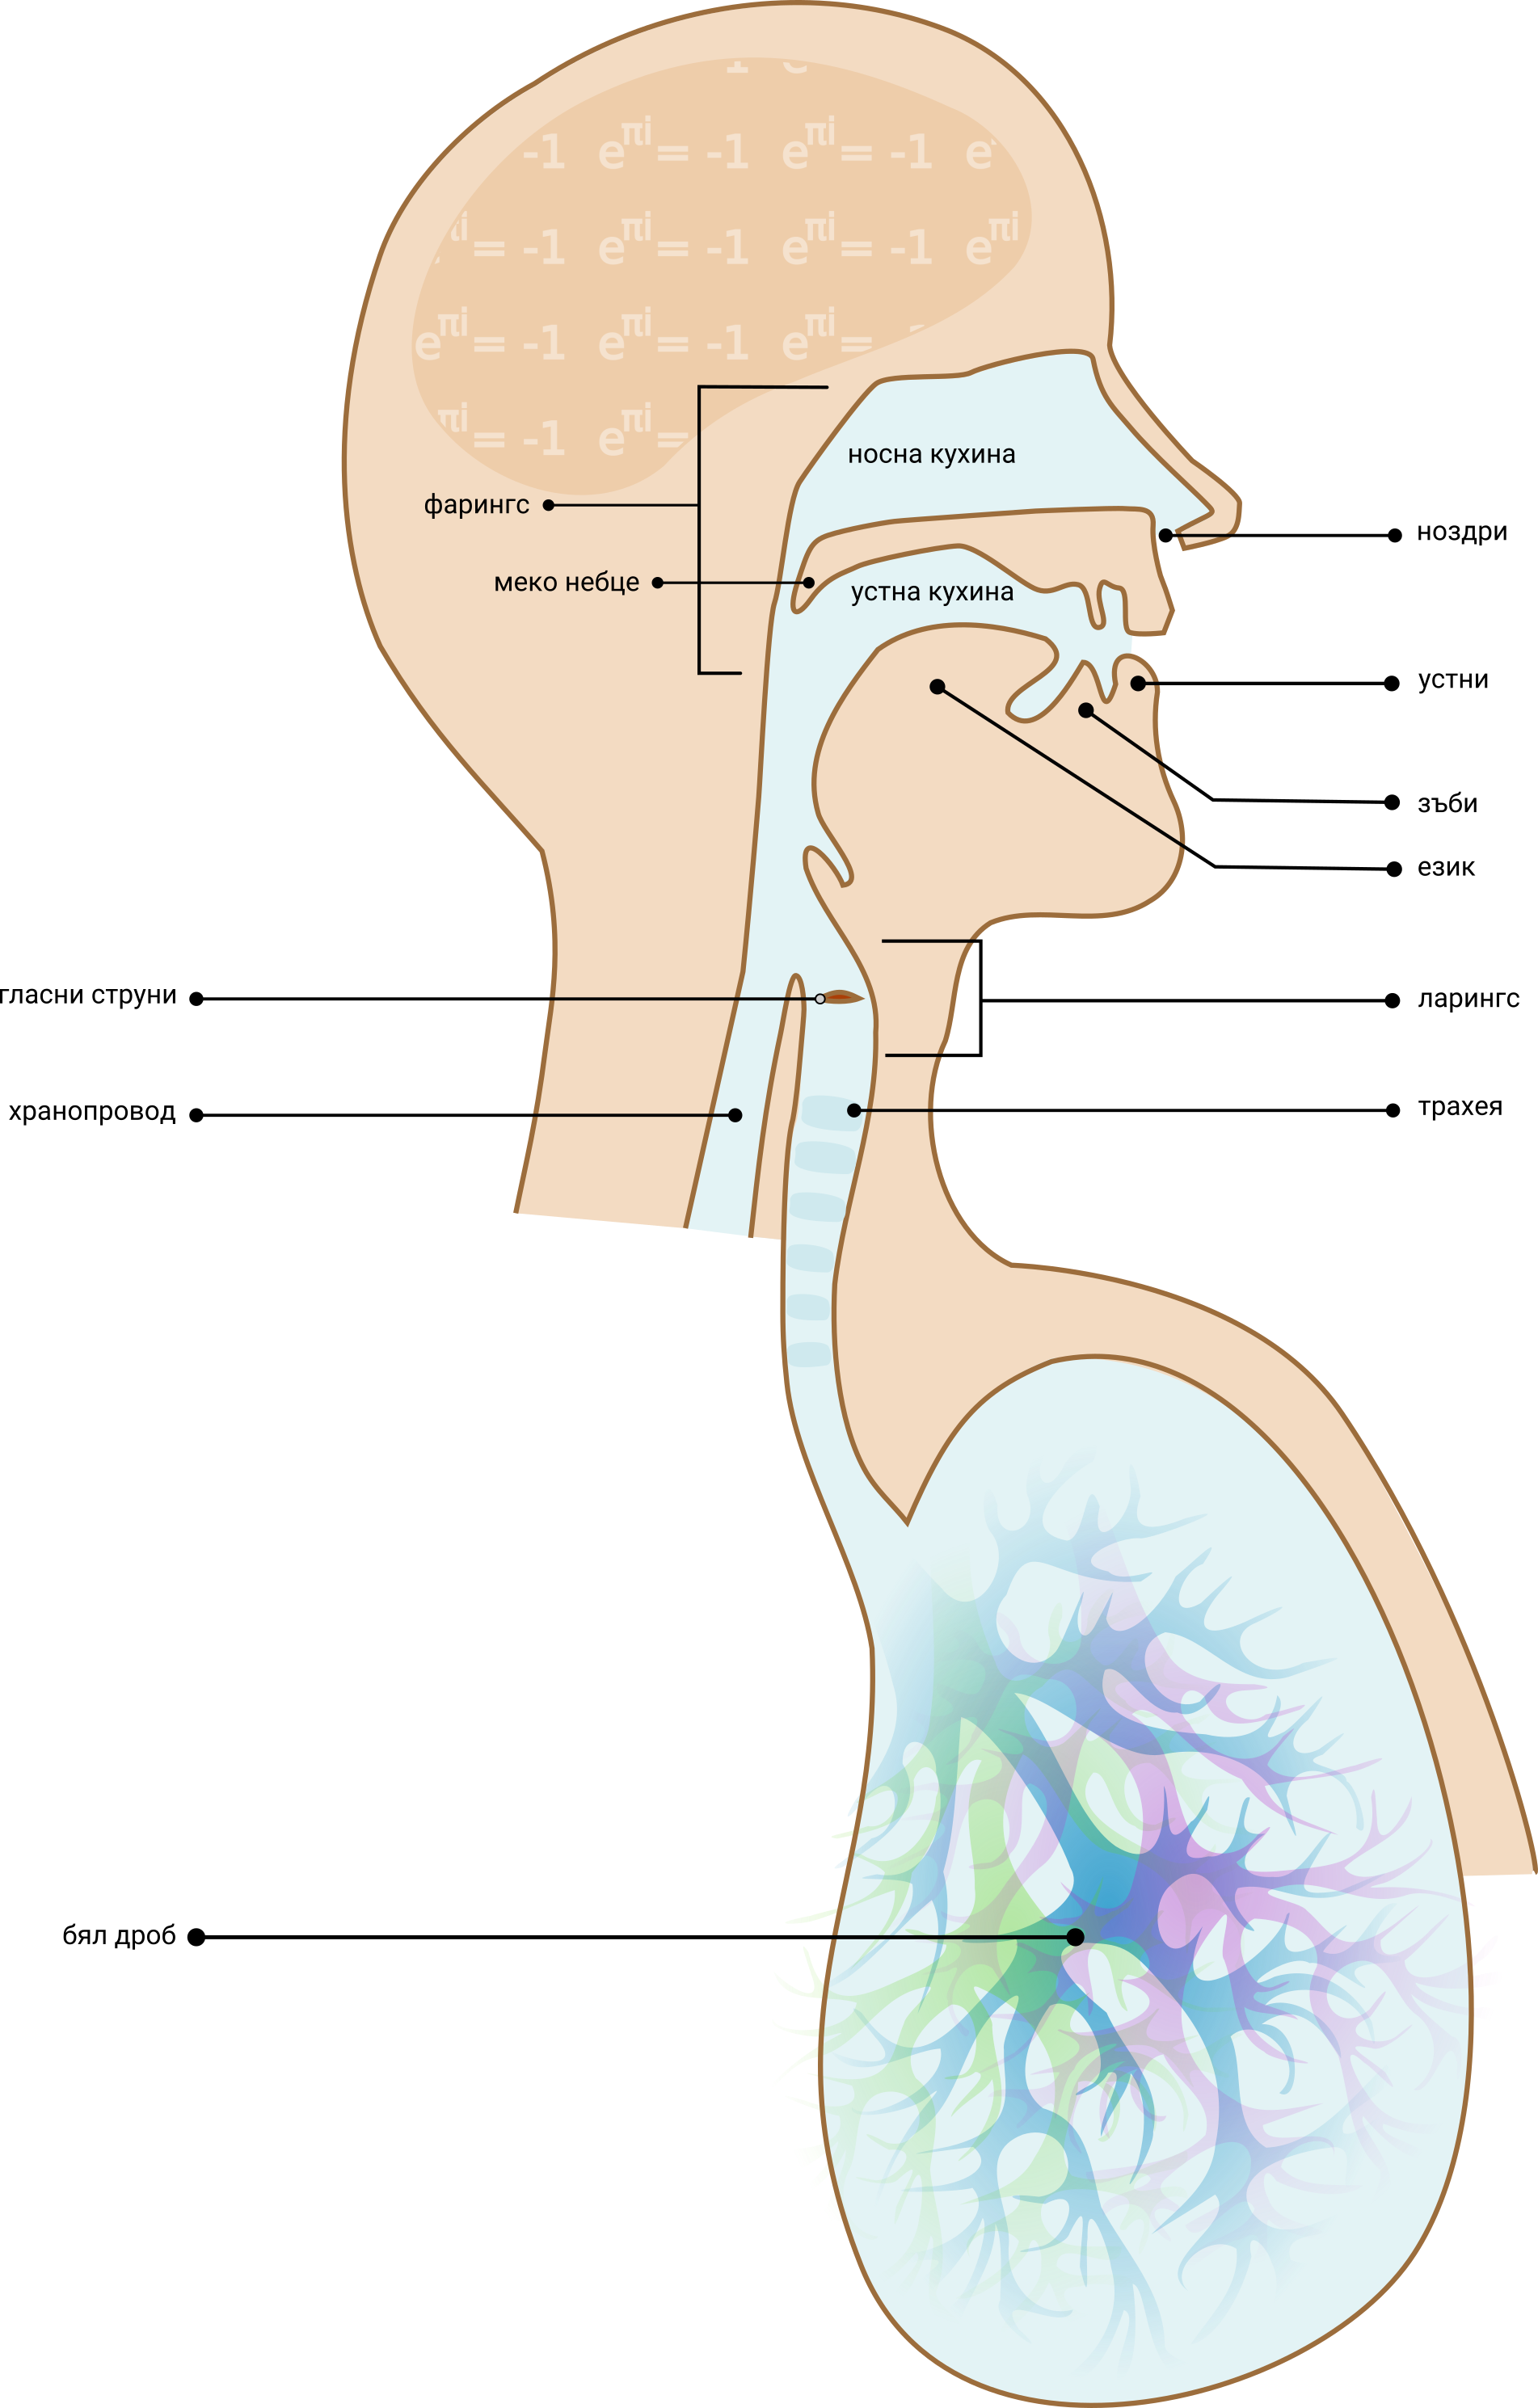
\includegraphics[width=0.48\paperwidth,valign=t]{physics}}%
            }
        \end{changemargin} 

        \caption{Система за производство на реч}%
        \label{fig:physics:1}
    \end{figure}
    
    Да разгледаме по-подробно $\autoref{fig:physics:1:a}$ и цялостна система за производство на реч.
    Речта, всъщност, представлява просто акустичната вълна, получена на края на системата - устни и ноздри - в следствие на изкарания от белия дроб въздух.

    Белият дроб работи като енергиен източник за тази системата - въздушният поток, получен при свиването му от междуребрените мускули и диафрагмата,
    се пропагира нагоре по трахеята и през глотиса (отворе между гласните струни). Тъй като налягането в глотиса е по-малко от това в който и да е от двата му края, по закона на Бернули
    в някакъв момент става толкова ниско, че позволява на гласните струни да се затворят. В следствие се натрупва налягане зад гласните струни, което в някакъв момент ги принуждава
    да се отворят и цикълът се повтаря отначало. В резултат се получава осцилиране на гласните струни. Честотата на отварянето и затварянето зависи от анатомични особености като еластичността и големината на
    гласните струни, налягането в белия дроб и други. При мъжете тази честота е средно 125 Hz, а при жените - 210 Hz. Акустичната вълна, която се получава в следствие на осцилацията,
    преминава през вокалния тракт, където се завихря, при срещане на прегради, като устни и зъби, и в крайна сметка напуска системата през някой от отворите.

    При целият този процес се губи част от енергията, поради различни фактори: стените на вокалния тракт са меки и еластични, радиацията на вълната при устните и ноздрите и други.

    В зависимост от начинът, по който вълната напуска системата, можем да класифицираме произведените звуци по следния начин:

    \begin{enumerate}
        \item Озвучени 
        При тези звуци гласните струни осцилират квази-периодично.
        \item Проходни (фрикативни) 
        При образуването на проходни звуци, вълната среща преграда по пътя си
            (като например зъби, устни), и се получава турболенция при опита въздухът да бъде избутан през преградата
        \item Преградни (експлозивни)
        Те се получават, когато преградата е пълна, което позволява да се натрупа налягане
        зад съответната прегада, което се освобождава рязко.
    \end{enumerate}
    
    Ако разгледаме вокалния тракт и носната кухина като свързани тръби с непостоянно напречно сечение и вземем предвид горното описание за генериране на звук,
    то честотният спектър ще зависи от честнотната пропускливост на тръбите (frequency selectivity) Трябва да видя онова в тетрадката. Това много прилича на свирене на духов инструмент.
    Честотите на които се получава резонанс зависи от формата и размера на тръбите. Известно е, че за да се образува определен звук, трябва да се промени формата на вокалния тракт по 
    съответния начин. (Например, когато човек казва "н" езикът се залепя зад зъбите и т.н.). В такъв случай, спектралните особености на сигнала се менят с времето, тъй като се мени и
    положението на вокалния тракт. Смята се [], че състоянието на вокалния тракт е сравнително статично (достатъчно статично за нашите цели) в рамките на 15ms, преди да се смени съответната
    фонема, която се изговаря. В такъв случай, можем да излседваме спектралните свойства в този отрязък от време и да извличаме информацията за подлежата емоция в него. 

    \section{Приближаване с тръби}
    За улеснение, нека разгледаме конкретна конфигурация. Например тази, при произнасянето на фонемата ``ъ'',тъй като е възможно най-проста.
    
    В случая на гласната ``ъ'' , глотиса трепти, а клапата към носната кухина е затворена и само устната кухина участва в образуването на звука. 
    Т.е. имаме някакъв източник на псевдо-периодично трептене $g$ - глотис, после вълната преминава и се променя от вокалния тракт $v$ и накрая излиза и се пречупва през
    устните $r$. Сигналът, който получаваме накрая е резултат от прилагането на филтъра на вокалния тракт и устните върху сигнала от глотиса.
    Това може да се запише като конволюция във времевия домейн. $y(t) = g(t)\ast v(t)\ast r(t)$ или произведение в
    честотния $\mathcal{Y}(\mathcal{z}) = \mathcal{G}(\mathcal{z}) \mathcal{V}(\mathcal{z}) \mathcal{R}(\mathcal{z})$, където
    \begin{flalign*}
    & \mathcal{G}(\mathcal{z}) = \mathcal{Z}\{g(t)\} && \\
    & \mathcal{V}(\mathcal{z}) = \mathcal{Z}\{v(t)\} && \\
    & \mathcal{R}(\mathcal{z}) = \mathcal{Z}\{r(t)\} && \\
    & \mathcal{Y}(\mathcal{z}) = \mathcal{Z}\{y(t)\} &&
    \end{flalign*}
    
   Това, от което се интересуваме, е $\mathcal{V}$.
    \begin{figure}[ht]%
        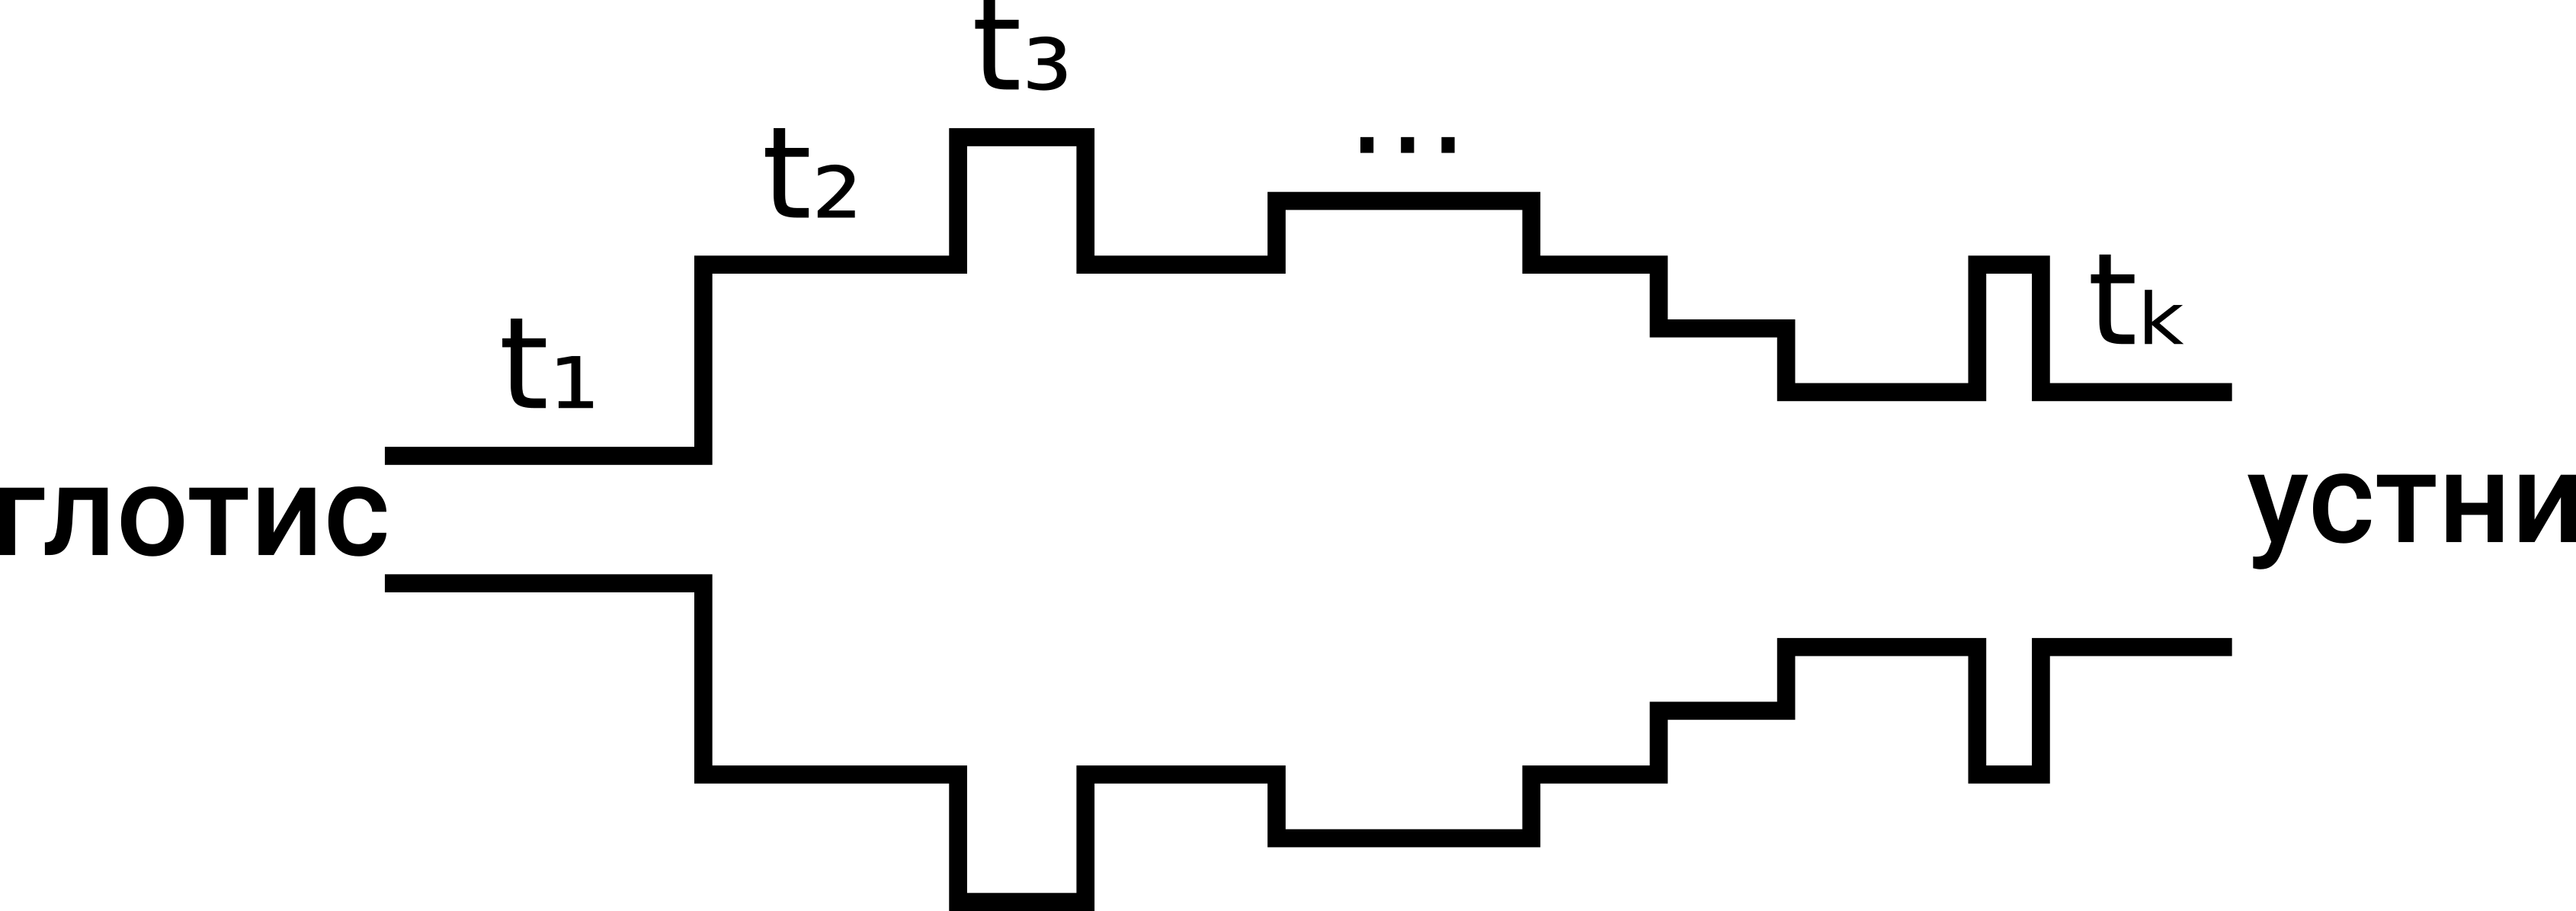
\includegraphics[width=\textwidth]{vocal_tubes}%
        \caption{Приближение на вокалния тракт с $N$ тръби}%
        \label{fig:2:2:1}
    \end{figure}

    Нека устната кухина е приближена с $N$ на брой тръби с постоянно напречно сечение, както е показано на $\autoref{fig:2:2:1}$
    За още по-голямо опростяване нека няма и загуба на енергия, каквата би се получила попринцип.

    Нека въведем следните стандартни означения:
    \begin{enumerate}
        \item{$\mathcal{c}$} - скорост на звука , т.е. това е разстоянието, което пропътува вълната за единица време
        \item{$\rho$} - плътност на въздуха
        \item{$A$} - напречно сечение
        \item{$u$} - обемна скорост
        \item{$p$} -  налягане - можем да си мислим за него като ``колко сила е нужна, за да се преместят частитицитe
    \end{enumerate}
    
    Нека означим с $u_L$ обемната скорост в последната точка на последната тръба $t_N$, тоест $u_L(t) = u_N(l_N, t)$, тъй като тя отговаря за изхода при усните, 
    а с $u_G$ обемната скорост съответстваща първата точка на $t_1$, тоест $u_G(t) = u_1(0, t)$, макар това да е изпълнено само в идеалния случай.
    Тогава можем да опишем отношението на $u_L$ и $u_G$ по следния начин: обемната скорост при усните е резултат от прилагането на филтъра на вокалния тракт върху сигнала
    от глотиса  $u_L(t) = u_G(t)\ast v(t) \longleftrightarrow v(t) = \cfrac{u_L}{u_G}$.
    Или изразено в честотния домейн като:
    \[
        \mathcal{V} = \cfrac{\mathcal{U}_L}{\mathcal{U}_G}
    \]

    Първо да разгледаме връзката между две съседни тръби.
    
    \subsection{Преминаване от една тръба в друга}

    Тъй като въздухът е течна среда, как пътува вълна през него се определя от свойствата на въздуха и от ограниченията на тръбата като дължина и ширина. Звуковите вълни, преминаващи през
    тръба изпълняват уравнения [Rabiner and Schafer, pg 59, (3.2a) (3.2b)]:
    
    \begin{subequations}
        \label{eq:tubes:01}
        \begin{align}
            \label{eq:tubes:01:a} \frac{\partial\rho}{\partial x} & = \frac{\rho}{A} \frac{\partial u}{\partial t}\\
            \label{eq:tubes:01:b} \frac{\partial u}{\partial x} & = \frac{A}{\rho \mathcal{c}^2} \frac{\partial \rho}{\partial t}
        \end{align}
    \end{subequations}

    При преминава от една тръба в друга, част от вълните ще преминат към следващата тръба, а част от тях ще се отразят в наобратно.
    В такъв случай във всеки момент от време $t$ и във всяка точка $x$ на всяка тръба,
    обемната скорост $u$ ще зависи от обемната скорост на вълните,
    които вървят ``напред'' и тази на вълните, които вървят ``назад''.
    Затова може да се покаже, че уравненията $\eqref{eq:tubes:01}$ имат решение във следния вид:

    \begin{subequations}
        \label{eq:tubes:02}
        \begin{align}
            u_{k}(x, t) & = \Q{u_{k}^{+}\B{t - \cfrac{x}{\mathcal{c}}} - u_{k}^{-}\B{t + \cfrac{x}{\mathcal{c}}}}\\
            p_{k}(x, t) & = \cfrac{\rho \mathcal{c}}{A_{k}} \Q{u_{k}^{+}\B{t - \cfrac{x}{\mathcal{c}}} + u_{k}^{-}\B{t + \cfrac{x}{\mathcal{c}}}}
        \end{align}
    \end{subequations}

    където 
    \begin{enumerate}
        \item{$t_{k}$} е $k$-тата тръба, която има дължина $l_k$ и лице на напречното сечение $A_k$
        \item{$x$} е разстояние в $t_k$ ($0\leq x \leq l_k$)
        \item{$t$} е момент от време
        \item{$u^{+}$ и $u^{-}$} са съответно вълните, които вървят "напред" и тези, които вървят "назад"
    \end{enumerate}

    Освен това, при преминаването от една тръба в друга са изпълнени следните равенства:
    \begin{subequations}
        \label{eq:tubes:03}
        \begin{align}
            u_k(l_k, t) & = u_{k+1}(0, t)\\
            p_k(l_k, t) & = p_{k+1}(0, t)
        \end{align}
    \end{subequations}

    Когато заместим уравнения $\eqref{eq:tubes:03}$ в $\eqref{eq:tubes:02}$, получаваме:
    \begin{flalign*}
        & u_k^+\B{t - \cfrac{l_k}{\mathcal{c}}} - u_k^{-}\B{t + \cfrac{l_k}{\mathcal{c}}} = u_{k+1}^{+}(t) - u_{k+1}^{-}(t) &&
        & \intertext{и}
        & \cfrac{\rho \mathcal{c}}{A_{k}} \Q{u_{k}^{+}\B{t - \cfrac{l_k}{\mathcal{c}}} + u_{k}^{-}\B{t + \cfrac{x}{\mathcal{c}}}} = \cfrac{\rho \mathcal{c}}{A_{k+1}} \Q{u_{k+1}^{+}(t) + u_{k+1}^{-}(t)} && \\
        & \iff && \\
        & \cfrac{A_{k+1}}{A_{k}}\Q{u_{k}^{+}\B{t - \cfrac{l_k}{\mathcal{c}}} + u_{k}^{-}\B{t + \cfrac{x}{\mathcal{c}}}} = u_{k+1}^{+}(t) + u_{k+1}^{-}(t) &&
    \end{flalign*}


    Нека означим с $\tau_{k}$ времето, за което вълна пропътува дължината на $k$-тата тръба, тоест $\tau_{k}= \cfrac{l_k}{\mathcal{c}}$. Тогава имаме:

    \begin{align}
        \label{eq:tubes:04}
        & u_k^+(t - \tau_k) - u_k^{-}(t + \tau_k) = u_{k+1}^{+}(t) - u_{k+1}^{-}(t)\\
        \label{eq:tubes:05}
        & \frac{A_{k+1}}{A_{k}}[u_{k}^{+}(t - \tau_k) + u_{k}^{-}(t + \tau_k)] = u_{k+1}^{+}(t) + u_{k+1}^{-}(t)
    \end{align}

    Първо, нека да изразим скоростта на вълните, които вървят "напред"
    в $(k+1)$-та тръба ($u_{k+1}^{+}$), чрез тези, които са преминали от предната тръба ($u_k^{+}$)
    и тези, които се отразяват от текущата ($u_{k+1}^{-}$).
    \begin{flalign}
        & \nonumber \intertext{От $\eqref{eq:tubes:04}$ получаваме}
        & \label{eq:tubes:06} u_{k}^{-}(t + \tau_{k}) = u_{k}^{+}(t - \tau_k) - u_{k+1}^{+}(t)  + u_{k+1}^{-}(t) && \\
        & \nonumber \intertext{Заместваме $\eqref{eq:tubes:06}$ в $\eqref{eq:tubes:05}$}
        & \nonumber u_{k+1}^{+}(t) = \frac{A_{k+1}}{A_k} u_{k}^{+}(t - \tau_k) + \frac{A_{k+1}}{A_k}[u_{k}^{+}(t - \tau_k) - u_{k+1}^{+}(t)  + u_{k+1}^{-}(t)] - u_{k+1}^{-}(t)  && \\
        & \nonumber u_{k+1}^{+}(t)\Q{1 + \frac{A_{k+1}}{A_k}} = u_{k}^{+}(t - \tau_k)\frac{2A_{k+1}}{A_k} + u_{k+1}^{-}(t)\Q{\frac{A_{k+1}}{A_k} - 1}  && \\
        & \nonumber u_{k+1}^{+}(t)\Q{\frac{A_k + A_{k+1}}{A_k}} = u_{k}^{+}(t - \tau_k)\frac{2A_{k+1}}{A_k} + u_{k+1}^{-}(t)\Q{\frac{A_{k+1} - A_k}{A_k}} && \\
        & \label{eq:tubes:07} u_{k+1}^{+}(t) = u_{k}^{+}(t - \tau_k)\Q{\frac{2A_{k+1}}{A_k + A_{k+1}}} + u_{k+1}^{-}(t)\Q{\frac{A_{k+1} - A_k}{A_k + A_{k+1}}} &&
    \end{flalign}

    Коефициентът, който стои пред $u_k^{+}(t - \tau_k)$ в уравнение $\eqref{eq:tubes:07}$,
    представлява количеството енергия, която преминава от тръба $k$ в тръба $k+1$,
    идваща от вълните, които се движат "напред" в $k$-тата тръба. Затова
    \begin{equation}
        \label{eq:tubes:08}
        t_k = \frac{2A_{k+1}}{A_k + A_{k+1}}
    \end{equation}

    се нарича \textbf{коефициент на преминаване} за $k$-тия преход (преходът между тръби $k$ и $k+1$).
    Коефициентът пред $u_{k+1}^{-}(t)$ представлява количестото енергия, получена от вълните,
    които вървят "назад" в тръба $k+1$. Затова 
    \begin{equation}
        \label{eq:tubes:09}
        r_k = \frac{A_{k+1} - A_k}{A_k + A_{k+1}}
    \end{equation}
    се нарича \textbf{коефициент на отрязяване} за $k$-тия преход. 
    
    Можем да забележим, че в специалния случай, в който напречните сечения на
    две съседни тръби са равни ($A_k = A_{k+1}$), би следвало всички
    вълни да преминават свободно. Наистина, ако заместим в уравнение $\eqref{eq:tubes:09}$,
    $r_k = 0$, a от $\eqref{eq:tubes:08}$ се вижда, че $t_k = 1$

    Нека изразим скоростта на вълните в тръба $k$ чрез скоростта на вълните в $(k+1)$-вата тръба. 
    

    \begin{subequations}
        \label{eq:tubes:10}
        \begin{flalign}
            & \nonumber \intertext{Първо разместваме уравнение $\eqref{eq:tubes:07}$}
            &  u_k^{+}(t - \tau_k) = u_{k+1}^{+}(t)\Q{\frac{A_k + A_{k+1}}{2A_{k+1}}} + u_{k+1}^{-}(t)\Q{\frac{A_k - A_{k+1}}{2A_{k+1}}} \label{eq:tubes:10:a} && \\
            & \nonumber \intertext{Заместваме $\eqref{eq:tubes:10:a}$ в $\eqref{eq:tubes:04}$}
            & \nonumber u_k^{-}(t + \tau_k) = u_k^{+}(t - \tau_k) - u_{k+1}^{+}(t) + u_{k+1}^{-}(t) && \\
            & \nonumber u_k^{-}(t + \tau_k) = u_{k+1}^{+}(t)\Q{\frac{A_k + A_{k+1}}{2A_{k+1}}} + u_{k+1}^{-}(t)\Q{\frac{A_k - A_{k+1}}{2A_{k+1}}} - u_{k+1}^{+}(t) + u_{k+1}^{-}(t) && \\
            & \nonumber u_k^{-}(t + \tau_k) = u_{k+1}^{+}(t)\Q{\frac{A_k + A_{k+1} - 2A_{k+1}}{2A_{k+1}}} + u_{k+1}^{-}(t)\Q{\frac{A_k - A_{k+1} + 2A_{k+1}}{2A_{k+1}}} && \\
            & \label{eq:tubes:10:b} u_k^{-}(t + \tau_k) = u_{k+1}^{+}(t)\Q{\frac{A_k - A_{k+1}}{2A_{k+1}}} + u_{k+1}^{-}(t)\Q{\frac{A_k + A_{k+1}}{2A_{k+1}}} &&
        \end{flalign}
    \end{subequations}

    Използвайки, че
    \begin{flalign*}
        \cfrac{1}{1 + r_k} & = \cfrac{A_k + A_{k+1}}{A_{k+1} - A_k + A_{k+1} + A_k} = \cfrac{A_k + A_{k+1}}{2A_{k+1}} && \\
        \\
        \cfrac{r_k}{1 + r_k} & = \cfrac{(A_{k+1} - A_k)}{(A_k + A_{k+1})} \cfrac{(A_k + A_{k+1})}{2A_{k+1}} = \cfrac{A_{k+1} - A_k}{2A_{k+1}}, &&
    \end{flalign*}
    можем да запишем уравненията $\eqref{eq:tubes:10}$ във вида:

    \begin{subequations}
        \label{eq:tubes:11}
        \begin{align}
           & u_k^{+}(t - \tau_k) = \cfrac{1}{1 + r_k} u_{k+1}^{+}(t) - \cfrac{r_k}{1+r_k} u_{k+1}^{-}(t)\\
           & u_k^{-}(t + \tau_k) = - \cfrac{r_k}{1+r_k} u_{k+1}^{-}(t) + u_{k+1}^{+}(t) + \cfrac{1}{1 + r_k} u_{k+1}^{-}(t)
        \end{align}
    \end{subequations}

    Сега да разгледаме уравнения $\eqref{eq:tubes:11}$ в $\mathcal{z}$-домейна:
    \begin{subequations}
        \label{eq:tubes:12}
        \begin{align}
            & \nonumber \mathcal{z}^{-\tau_k}U_k^{+}(\mathcal{z}) = \cfrac{1}{1 + r_k} U_{k+1}^{+}(\mathcal{z}) - \cfrac{r_k}{1+r_k} U_{k+1}^{-}(\mathcal{z}) \\
            & \nonumber \mathcal{z}^{\tau_k} U_k^{-}(\mathcal{z}) = - \cfrac{r_k}{1+r_k} U_{k+1}^{-}(\mathcal{z}) + U_{k+1}^{+}(\mathcal{z}) + \cfrac{1}{1 + r_k} U_{k+1}^{-}(\mathcal{z}) \\
            & U_k^{+}(\mathcal{z}) = \cfrac{\mathcal{z}^{\tau_k}}{1 + r_k} U_{k+1}^{+}(\mathcal{z}) - \cfrac{r_k\mathcal{z}^{\tau_k}}{1+r_k} U_{k+1}^{-}(\mathcal{z})\\
            & U_k^{-}(\mathcal{z}) = - \cfrac{r_k\mathcal{z}^{-\tau_k} }{1+r_k} U_{k+1}^{-}(\mathcal{z}) + U_{k+1}^{+}(\mathcal{z}) + \cfrac{\mathcal{z}^{-\tau_k} }{1 + r_k} U_{k+1}^{-}(\mathcal{z})
        \end{align}
    \end{subequations}

    \subsection{Ограничения при устните}
    Както се вижда от фигура \autoref{fig:2:2:1}, изходът при устните представлява отвор, който
    пречупва радииращите звуковите вълни.
    За да се опишат ефектите от това пречупване, е нужно да знаем връзката между
    налягането и обемната скорост. В реалния случай това би било трудно, затова за улеснение
    ще приемем, че изходът при устните е преграден от безкрайна равнина. В такъв случай може
    да се покаже, че е изпълнено:
    \begin{equation}
        \label{eq:tubes:13}
        \mathcal{P}_L(\mathcal{z}) = Z_L(\mathcal{z}) \mathcal{U}_L(\mathcal{z}),
    \end{equation}
    където 
    $Z_L(\mathcal{z})$ се нарича радиационен импеданс (пълно съпротивление), описва загубите, които се получават на изхода, и има вида:
    \[
        Z_L(\mathcal{z}) = \cfrac{j\mathcal{z} L_r R_r}{R_r + j\mathcal{z} L_r},    
    \]
    Където $\mathcal{z}$ е честота, $L_r$ и $R_r$ са константи, определени от размера на отвора на устата. За практически цели се избират:

    \begin{multicols}{2}
        \begin{equation*}
          R_r = \cfrac{128}{9\pi^2} > 1
        \end{equation*}\break
        \begin{equation*}
          L_r = \cfrac{8a}{3\pi \mathcal{c}}
        \end{equation*}
      \end{multicols}
    $a$ - радиус на отвора, $\mathcal{c}$ - скоростта на звука.

    При много ниски честоти $Z_L(\mathcal{z}) \approx 0$, което значи, че съпротивлението на устните е почти нулево.
    При средни честоти ($\mathcal{z}L_r \ll R_r$), $Z_L(\mathcal{z}) \approx j\mathcal{z}L_r$, а високи честоти, ($\mathcal{z}L_r \gg R_r$) $Z_L(\mathcal{z}) \approx R_r$. 
    Това значи, че загубите при устните са най-големи при големи честоти, тъй като тогава импедансът е най-голям.

    В случая, в който честотата $\mathcal{z}$ е висока, $Z_L \approx R_r$ е реално число  и не зависи от $\mathcal{z}$. Тогава можем да разгледаме уравнението $\eqref{eq:tubes:13}$ във
    времевия домейн, ще получим:
    \begin{flalign*}
        & p_L(t) = Z_L u_L(t) && \\
        & \cfrac{\rho\mathcal{c}}{A_L}\Q{u_N^{+}(t - \tau_N) + u_N^{-}(t + \tau_N)} = Z_L\Q{u_N^{+}(t - \tau_N) - u_N^{-}(t + \tau_N)} &&\\
        & u_N^{-}(t + \tau_N) \cfrac{(\rho\mathcal{c} + A_L Z_L)}{A_L} = u_N^{+}(t - \tau_N) \cfrac{(A_L Z_L - \rho\mathcal{c})}{A_L} &&\\
        & u_N^{-}(t + \tau_N) = -r_L u_N^{+}(t - \tau_N), \text{ където}&&
    \end{flalign*}
    \begin{equation}
        \label{eq:tubes:14}
        r_L = \B{\frac{\rho\mathcal{c} - A_L Z_L}{\rho\mathcal{c} + A_L Z_L}}
    \end{equation}

    Като заместим в уравнение $\eqref{eq:tubes:01:b}$, получаваме
    \begin{flalign}
       \label{eq:tubes:15}
       \nonumber u_N(l_N, t) = u_N^{+}(t - \tau_N) - u_N^{-}(t + \tau_N) & =  &&\\
       & = (1 + r_L) u_N^{+}(t - \tau_N) &&
    \end{flalign}

    В случая, в който $Z_L \approx j\mathcal{z}L_r$ е комплексно, може да се покаже, че уравнение \eqref{eq:tubes:14} остава в сила,
    но в този случай и $r_L$ също ще бъде комплексно.

    \subsection{Ограничения при глотиса}

    Както при устните, така и при глотиса, трябва да се отчете импедансът. Например, трябва да се отчете фактът,
    че когато глотисът е затворен, импедансът е безкраен, а обемната скорост нулева.
    Връзката $U_1(0, \mathcal{z}) = U_G(\mathcal{z})$, която използвахме досега,
    е твърде наивна, затова едно по-добро приближение би било:
    \begin{align}
    \label{eq:tubes:16}
        U(0, \mathcal{z}) =  U_G(\mathcal{z}) - \frac{P(0, \mathcal{z})}{Z_G(\mathcal{z})},
    \end{align}
    където $Z_G$ описва импеднса на глотиса и $Z_G(\mathcal{z}) = R_G + j \mathcal{z} L_G,$
    
    $L_G, R_G - $константи
    Отново предполагайки, че $Z_G$ е реално, тоест честотата $\mathcal{z}$ е много ниска, можем да разгледаме
    уравнение $\eqref{eq:tubes:16}$ във времевия домейн:
    \begin{flalign}
        \label{eq:tubes:17}
        & \nonumber u_1^{+}(t) - u_1^{-}(t) = u_G(t) - \frac{\rho \mathcal{c}}{A_1}\Q{\frac{u_1^{+}(t) + u_1^{-}(t)}{Z_G}} && \\
        & \nonumber u_1^{+}(t)\Q{1 + \frac{\rho\mathcal{c}}{A_1 Z_G}}  = u_G(t) + u_1^{-}(t)\Q{1 - \frac{\rho\mathcal{c}}{A_1 Z_G}} && \\
        & \nonumber u_1^{+}(t) = u_G(t)\Q{\frac{A_1 Z_G}{A_1 Z_G + \rho \mathcal{c}}} + u_1^{-}(t)\Q{\frac{A_1 Z_G - \rho \mathcal{c}}{A_1 Z_G + \rho \mathcal{c}}} &&\\
        & \nonumber u_1^{+}(t) = u_G(t) \Q{\frac{1 + r_G}{2}} + r_G u_1^{-}(t)&& \\
        & U_G(\mathcal{z}) = \Q{\frac{2}{1 + r_G}}U_1^{+}(\mathcal{z}) - \Q{\frac{2r_G}{1 + r_G}}U_1^{-}(\mathcal{z}), \text{където} &&
    \end{flalign}
    \begin{equation*}
        r_G = \B{\cfrac{A_1 Z_G - \rho\mathcal{c}}{A_1 Z_G + \rho\mathcal{c}}}
    \end{equation*}
    и използвайки, че
    \begin{flalign*}
        \cfrac{1 + r_G}{2} & = \cfrac{A_1Z_G + \rho\mathcal{c} + A_1Z_G - \rho\mathcal{c}}{2(A_1Z_G + \rho\mathcal{c})} = \cfrac{A_1Z_G}{A_1Z_G + \rho\mathcal{c}} && \\
    \end{flalign*}

    Отново може да се покаже, че ако $Z_G$ е комплексно, уравнението $\eqref{eq:tubes:18}$ е в сила и
    в този случай $r_G$ също е комплексно.
    За улеснение обикновено $Z_L$ и $Z_G$ се взимат реални. 

    \subsection{Общ вид на $\mathcal{V}$}
    За да видим общия вид на $\mathcal{V}$, нека всички тръби имат равна дължина и $\tau_i = \frac{1}{2}, i \in[1...N]$
    Тогава уравнения $\eqref{eq:tubes:12}$ имат вида:
    
    \begin{subequations}
        \label{eq:tubes:18}
        \begin{align}
            & U_k^{+}(\mathcal{z}) = \cfrac{\mathcal{z}^{1/2}}{1 + r_k} U_{k+1}^{+}(\mathcal{z}) - \cfrac{r_k\mathcal{z}^{1/2}}{1+r_k} U_{k+1}^{-}(\mathcal{z})\\
            & \nonumber \\
            & U_k^{-}(\mathcal{z}) = - \cfrac{r_k\mathcal{z}^{-1/2} }{1+r_k} U_{k+1}^{-}(\mathcal{z}) + U_{k+1}^{+}(\mathcal{z}) + \cfrac{\mathcal{z}^{-1/2} }{1 + r_k} U_{k+1}^{-}(\mathcal{z})
        \end{align}
    \end{subequations}

    За да опишем граничните условия при устните, ще приемем, че $U_{N+1}(\mathcal{z})$ е $\mathcal{z}$-трансформацията
    на входа на $(N+1)$-та тръба, която е безкрайно дълга, и заради това скоростта на вървящите ``назад'' вълни трябва да бъде 0
    Тоест,
    \begin{align}
        \label{eq:tubes:19}
        & U_{N+1}^{+} (\mathcal{z}) = U_L(\mathcal{z})\\
        & \nonumber U_{N+1}^{-}(\mathcal{z}) = 0
    \end{align}

    Ако представим уравнения $\eqref{eq:tubes:18}$ в матричен вид, получаваме:

    $U_k = Q_k U_{k+1}$ за

    \begin{multicols}{2}
        $U_k = 
            \begin{bmatrix}
                U_k^{+}(\mathcal{z}) \\
                U_k^{-}(\mathcal{z}) \\
            \end{bmatrix}$
        \vfill
        \columnbreak
        $Q_k = 
            \begin{bmatrix}
                \cfrac{\mathcal{z}^{1/2}}{1 + r_k} & \cfrac{-r_k \mathcal{z}^{1/2}}{1 + r_k} \\
                & \\
                \cfrac{-r_k \mathcal{z}^{-1/2}}{1 + r_k} & \cfrac{\mathcal{z}^{-1/2}}{1 + r_k} \\
            \end{bmatrix}$
    \end{multicols}

    \begin{flalign*}
        & U_1 = Q_1 U_2 = Q_1 Q_2 U_3 = \cdots = Q_1 ... Q_N U_{N+1} = \Q{\prod_{i=1}^{N} {Q_i}}U_{N+1}
    \end{flalign*}

    Сега представяме уравнение $\eqref{eq:tubes:17}$ като
    \begin{flalign*}
        & U_G(\mathcal{z}) = \left[
            \begin{array}{cc}
                \cfrac{2}{1+r_G}, & -\cfrac{2r_G}{1 + r_G} \\
            \end{array}
        \right] U_1 &&\\
    \end{flalign*}

    Ограниченията за $\eqref{eq:tubes:19}$ за $U_L$ ни дават, че
    
    \begin{flalign*}
        & U_{N+1} = 
        \left[ \begin{array}{cc}
                U_{N+1}^{+}(\mathcal{z}) \\
                U_{N+1} ^{-}(\mathcal{z})
            \end{array}\right] = 
        \left[ \begin{array}{cc}
            U_L(\mathcal{z}) \\
            0
        \end{array}\right]= 
        \left[ \begin{array}{cc}
            1 \\
            0
        \end{array}\right] U_L(\mathcal{z}) && \\ 
    \end{flalign*}

    Тогава 

    \begin{flalign}
        \label{eq:tubes:20}
        & \frac{1}{\mathcal{V}(\mathcal{z})} = \frac{U_G(\mathcal{z})}{U_L(\mathcal{z})}  = \left[
            \begin{array}{cc}
                \cfrac{2}{1+r_G}, & -\cfrac{2r_G}{1 + r_G} \\
            \end{array}
            \right] \prod_{i=1}^{N} {Q_i} \left[ \begin{array}{cc}
                1 \\
                0
            \end{array}\right] &&
    \end{flalign}
            

    Нека изразим $Q_k$ по следния начин:
    
    \begin{flalign*}
        & Q_k = \left[\begin{array}{cc}
                \cfrac{\mathcal{z}^{1/2}}{1 + r_k} & \cfrac{-r_k \mathcal{z}^{1/2}}{1 + r_k} \\
                & \\
                \cfrac{-r_k \mathcal{z}^{-1/2}}{1 + r_k} & \cfrac{\mathcal{z}^{-1/2}}{1 + r_k} \\
            \end{array}\right] = 
            z^{1/2}\left[\begin{array}{cc}
                \cfrac{1}{1 + r_k} & \cfrac{-r_k}{1 + r_k} \\
                & \\
                \cfrac{-r_k \mathcal{z}^{-1}}{1 + r_k} & \cfrac{\mathcal{z}^{-1}}{1 + r_k} \\
            \end{array}\right] = 
            \mathcal{z}^{1/2} \hat{Q}_k && 
    \end{flalign*}

    Тогава уравнение $\eqref{eq:tubes:20}$ има вида


    \begin{flalign}
        \label{eq:tubes:21}
        & \frac{1}{\mathcal{V}(\mathcal{z})} = \frac{U_G(\mathcal{z})}{U_L(\mathcal{z})}  = \mathcal{z}^{N/2}\left[
            \begin{array}{cc}
                \cfrac{2}{1+r_G}, & -\cfrac{2r_G}{1 + r_G} \\
            \end{array}
            \right] \prod_{i=1}^{N} {\hat{Q}_i} \left[ \begin{array}{cc}
                1 \\
                0
            \end{array}\right] &&
    \end{flalign}
            
    Нека изразим общия вид на $\mathcal{V}(\mathcal{z})$. За $N=2$, например, $\eqref{eq:tubes:21}$ има вида:

    \begin{flalign}
    \label{eq:tubes:22}
    & \mathcal{V}(\mathcal{z}) = \frac{0.5 (1+r_G)\prod\limits_{i=1}^{2}(1 + r_i)\mathcal{z}^{-1}}{1 + (r_Gr_1 + r_1r_2)\mathcal{z}^{-1} + (r_Gr_2)\mathcal{z}^{-2}}, &&
    \end{flalign}
    както е показано в $\autoref{appendix:2:01}$

    За всяка стойност на $N$ в числител се получава произведение $(1 + r_G)\prod\limits_{i=1}^{N}(1 + r_i)$,a в знаменател се получава полином на $\mathcal{z}$ и от основната теорема на алгебрата следва, че уравнението $\eqref{eq:tubes:21}$ ще има решения от вида:

    \begin{align}
        \label{eq:tubes:23}
        \mathcal{V}(\mathcal{z}) = \frac{0.5(1+r_G)\prod\limits_{i=1}^{N}{(1 + r_i)} \mathcal{z}^{-N/2}}{1 - \sum\limits_{i=1}^{N}{\alpha_i \mathcal{z}^{-i}}}
    \end{align}

    \subsection{Общ вид на $\mathcal{R}$}

    За да моделираме устните, трябва да се отрази радиацията. Искаме за радиацията да е изпълнено $\autoref{eq:tubes:12}$, като
    \begin{flalign*}
        & \mathcal{R}(\mathcal{z}) = P_L(\mathcal{z}) U_L(\mathcal{z}) &&
    \end{flalign*}

    Също така видяхме, че налягането и скоростта са свързани с високочестотен филтър, следователно
    може да се опише от КИХ филтър, тоест:

    \begin{flalign}
        \label{eq:tubes:24}
        & \mathcal{R}(\mathcal{z}) = (1 - \gamma\mathcal{z} ^ {-1}) &&
    \end{flalign}

    \subsection{Общ вид на $\mathcal{G}$}

    За да се симулира действието на глотиса, трябва да отчетем как се държи той при
    изговаряне на различни видове звуци. При звучните, както описахме по-горе, глотисът
    произвежда квази-периодичен сигнал, а при беззвучните се получава случаен шум.

    Да разгледаме вида на $\mathcal{G}$ в случая на озвучен звук.
    \begin{figure}[ht]%
        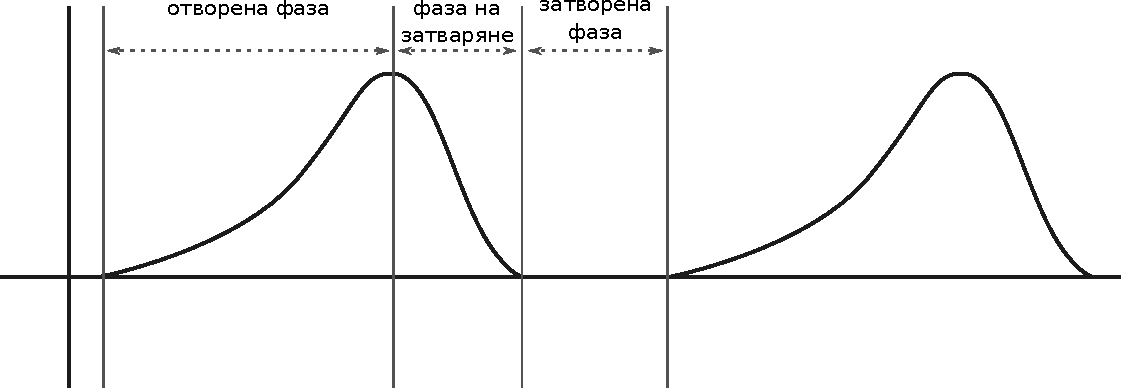
\includegraphics[width=\textwidth]{glotal_pulse}%
        \caption{Пример за импулс от глотиса}%
        \label{fig:2:2:2}
    \end{figure}
    
    На $\autoref{fig:2:2:2}$ се вижда, че импулсът от глотиса може да се раздели на три фази:
    \begin{enumerate}
        \item Отворена фаза с край $F_1$
        \item Фаза на затваряне с начало $F_1$ и край $F_2$
        \item Затворена фаза с начало $F_2$
    \end{enumerate}

    Съответно ще моделираме функцията $\mathcal{G}$ в зависимост от фазата. По-лесно ще е
    да се направи във времевия домейн. Едно добро приближение е:

    \begin{flalign*}
        & g(t) = 
        \begin{cases}
            \cfrac{1}{2}( 1 - \cos{(\pi n / F1)}), & 0\leq t \leq F_1\\
            \cos{(\pi(n - N_1)/2N_2)}, & F_1 \leq t \leq F_2\\
            0, & \text{иначе}   
        \end{cases}   &&     
    \end{flalign*}

    Тъй като функцията $g$ има краен брой точки, в които не е нула, $\mathcal{z}$-трансформацията ѝ
    ще има две нули. Тоест може да се моделира като:

    \begin{flalign}
        \label{eq:tubes:25}
        & \mathcal{G}(\mathcal{z}) = (1 - \beta_1 \mathcal{z}^{-1})(1 - \beta_2 \mathcal{z}^{-1}) &&
    \end{flalign}
    
    В случая на беззвучие за $\mathcal{G}$ се използва някакъв генератор на случайни числа, за да се симулира шум.

    \section{Общ вид на $\mathcal{H}$}
    От уравнения $\ref{eq:tubes:22}, \ref{eq:tubes:24}, \ref{eq:tubes:25}$ следва, че видът на  $\mathcal{H}$ е
    \begin{flalign}
        \label{eq:tubes:26}
        & \mathcal{Y}(\mathcal{z}) = \mathcal{G}(\mathcal{z})\mathcal{V}(\mathcal{z})\mathcal{R}(\mathcal{z}) = (1 - \beta_1 \mathcal{z}^{-1})(1 - \beta_2 \mathcal{z}^{-1})(1 - \gamma\mathcal{z} ^ {-1})\cfrac{0.5(1+r_G)\prod\limits_{i=1}^{N}{(1 + r_i)} \mathcal{z}^{-N/2}}{1 - \sum\limits_{i=1}^{N}{\alpha_i \mathcal{z}^{-i}}} &&
    \end{flalign}

    \section{Представяне със системи}

    Нека имаме чистия сигнал от глотиса $g[t]$. При преминаването му през вокалния тракт и устните, той
    се променя, в следствие на различни фактори като турболенция, поглъщане, отрязяване, в следствие на което 
    на изхода (устните), получаваме сигналът $y[n]$.
    
    \begin{definition*}{Система}\\
    Механизъм, който манипулира един или повече сигнали с някаква цел до
    получаване на нов сигнал, се нарича система
    
    Обикновено в практическия свят се използват системи, чието действие е предварително известно (и желано). Такива системи
    наричаме \textbf{филтри}. Филтрите обикновено изпълняват някаква точно определена манипулация върху сигнала, например
    да премахват всички честоти под или над определа честота.
    \end{definition*}

    С $g[n] \mapsto y[n]$ ще бележим, че $y$ е отговорът на системата за вход $g$. В такъв случай, системата, която ще разгледаме, е тази на вокалния тракт. Ще ни интересуват
    няколко класа системи.

    \begin{definition*}{Линейна система}\\
        Ако $x_1[n] \mapsto y_1[n]$ и $x_2[n] \mapsto y_2[n]$, то системата е линейна $\longleftrightarrow$

        $ax_1[n] + bx_2[n] \mapsto ay_1[n] + by_2[n]$ 
    \end{definition*}
    

    \begin{definition*}{Времево-независима система}\\
        Нека $x[n] \mapsto y[n]$. Тогава, ако за всяко $n_0: x[n - n_0] \mapsto y[n - n_0]$, то
        системата е времево-независима.
    \end{definition*}

    Специален подклас на линейните, времево-независими системи, е класът на системите, удовлетворяващи диференчното уравнение от ред $N$
    с константни коефициенти:
    \begin{flalign}
        \label{eq:systems:1}
        & \sum\limits_{k=0}^{N} a_k y [n-k] = \sum\limits_{m=0}^{M}b_k x[n-m] &&
    \end{flalign}


    Вокалният тракт е времето независима система, защото изходът $y[n]$ не зависи от момента
    от време, а само от специфичната му конфигурация в текущия момент, т.е. положението на езика, устните,
    зъбите. 
    Нека предположим, че вокалния тракт е линейна, времево-независима система, която удовлетворява уравнение $\autoref{eq:systems:1}$, и да разгледаме свойствата.
    
    Искаме да опишем как работи тази система. За момента знаем как ще реагира тя, ако ѝ подадем входен сигнал $g[n]$.  
    Но вместо да разглеждаме отговора на системата за широк спектър от входни функции, ще е полезно да имаме характеризация,
    която не зависи от входа.
    
    Пъро да разгледаме входа по различен начин. Ако за всеки момент от време $n_0$ имаме импулси със сила $g[n_0]$, то можем да мислим за входния сигнал $g[n]$
    като за сума от тези импулси. Тоест, нека имаме дискретният единичен импулс:

    \begin{flalign*}
        &\delta[n] = \begin{cases}
        1, & n = 0\\
        0, & \text{иначе}\\
        \end{cases} &&
    \end{flalign*}

    Тогава можем да представим входния сигнал $g[n]$ като
    \begin{flalign*}
        & g[n] = \sum\limits_{k=-\infty}^{\infty} g[k]\delta[n-k] &&
    \end{flalign*}

    Нека $\delta[n-k] \mapsto h_k[n]$. Тъй като системата е линейна, е изпълнено че:
    \begin{flalign}
        \label{eq:systems:2}
        & g[n] = \sum\limits_{k=-\infty}^{\infty}g[k]\delta[n-k] \mapsto \sum\limits_{k = -\infty}^{\infty}g[k]h_k[n] = y[n] &&, 
    \end{flalign}

    Времевата инвариантност ни казва, че ако $\delta[n] \mapsto h[n]$, то $\delta[n -k] \mapsto h[n-k]$, следователно
    в случая на вокалния тракт $\autoref{eq:systems:2}$ има вида:

    \begin{flalign}
        \label{eq:systems:3}
        &  y[n] = \sum\limits_{k = -\infty}^{\infty}g[k]h_k[n] = \sum\limits_{k = -\infty}^{\infty}g[k]h[n-k] &&, 
    \end{flalign}

    \begin{definition*}{Дискретна конволюция}\\
        Ако $f, g: \mathbb{N} \mapsto \mathbb{Z}$,
        дискретна конволюция (конволюционна сума) на $f$ и $g$, наричаме
  
        $(f\ast g)[n] = \sum\limits_{k=-\infty}^{\infty} f[k]g[n-k]$
    \end{definition*}

    Тоест $y[n] = (g \ast h)[n]$
    Ако запишем това равенство в $\mathcal{z}$-домейна, получаваме
    \begin{flalign}
        \label{eq:systems:4}
        & \nonumber \mathcal{Y}(\mathcal{z}) = \mathcal{G}(\mathcal{z})\mathcal{H}(\mathcal{z}) &&\\
        & \mathcal{H}(\mathcal{z}) = \cfrac{\mathcal{Y}(\mathcal{z})}{\mathcal{G}(\mathcal{z})} &&
    \end{flalign}
    $\mathcal{H}$ се нарича предавателна функция за системата.

    Да разгледаме $\autoref{eq:systems:1}$ в $\mathcal{z}$-домейна.
    \begin{flalign}
        \label{eq:systems:5}
        & \nonumber\Q{\sum\limits_{k=0}^{N}a_k\mathcal{z}^{-k}}\mathcal{Y}(\mathcal{z}) = \Q{\sum\limits_{m=0}^{M} b_m \mathcal{z}^{-m}}\mathcal{G}(\mathcal{z}) &&\\
        & \cfrac{\mathcal{Y}(\mathcal{z})}{\mathcal{G}(\mathcal{z})} = \cfrac{\sum\limits_{m=0}^{M} b_m \mathcal{z}^{-m}}{\sum\limits_{k=0}^{N} a_k \mathcal{z}^{-k}} &&
    \end{flalign}

    Когато заместим $\autoref{eq:systems:5}$ в $\autoref{eq:systems:4}$, получаваме
    \begin{flalign}
        \label{eq:systems:6}
        & \mathcal{H}(\mathcal{z}) =  \cfrac{\sum\limits_{m=0}^{M} b_m \mathcal{z}^{-m}}{\sum\limits_{k=0}^{N} a_k \mathcal{z}^{-k}} &&
    \end{flalign}

    \section{Характеристики}
    \subsection{Избор}
    \subsection{Извличане}
        Първо се изчита wav файла, като данни се запазват в масив от float числа.
        Базирайки се на идеята, че вокалния тракт е статичен за много къс период от време,
        накъсваме масива с данните на отделни застъпващи се фреймове, в рамките на които сигналът е статичен ("представяме си, че е статичен"). За да получим добра
        добра честотна резолюция, трябва да се включат голям брой samples от файла, но колкото по-голяма е дължината
        на фрейма, толкова по-голям е шансът да включим данни за различни конфигурации на глотиса.
        За да се постигне някакъв trade-off между двете, обикновено стойностите, които се избират, са 
        25 милисекунди за дължина на фрейм и 10 милисекунди за разстояние между два последователни фрейма.[Paul]
        
        Тъй като алгоритъмът за извличане на mfcc коефициенти, изисква броя на самплите да е степен на 2,
        допълваме последните фреймове с 0, ако това е нужно, тъй като това не влияе на точността. [мжое би онази статия за fourier]

    \section{Класификация}    
    \section{Резултати}

\chapter{Грубо в мозъка}
    \section{Характеристики}
        \subsection{Избор}
        \subsection{Извличане}
    \section{Класификация}    
    \section{Резултати}
\chapter{Двойната звезда}
    \section{Резултати}
\chapter{Големият портрет}

\begin{appendices}

    \chapter{Приложение за полюси и нули}

    \section{Дефиниция}

    Нека $\mathcal{z} \in \mathbb{C}$. Видяхме,че предавателната функция $\mathcal{H}$ на определени системи (и в частност филтри) има вида
    \begin{flalign}
        \tag{\ref{eq:systems:6}}
        & \mathcal{H}(\mathcal{z}) =  \cfrac{\sum\limits_{m=0}^{M} b_m \mathcal{z}^{-m}}{\sum\limits_{k=0}^{N} a_k \mathcal{z}^{-k}} = && \\
        \nonumber & \mathcal{H}(\mathcal{z}) = \cfrac{N(\mathcal{z})}{D(\mathcal{z})} = G \cfrac{(\mathcal{z} - \beta_1)(\mathcal{z} - \beta_2)...(\mathcal{z} - \beta_M)}{(\mathcal{z} - \alpha_1)(\mathcal{z} - \alpha_2)...(\mathcal{z} - \alpha_N)}, &&
    \end{flalign}

    където $G = b_M/a_N$ и се нарича усилващ коефициент.

    С $\beta_i$ означаваме корените на уравнението $N(\mathcal{z}) = 0$. Те се наричат нули на системата и 
    $\lim\limits_{\mathcal{z} \rightarrow \beta_i} \mathcal{H}(\mathcal{z}) = 0$

    С $\alpha_i$ означаваме корените на уравнението $D(\mathcal{z}) = 0$. Те се наричат полюси на системата и 
    $\lim\limits_{\mathcal{z} \rightarrow \alpha_i} \mathcal{H}(\mathcal{z}) = \infty$

    Тъй като коефициентите на $N(\mathcal{z})$ и $D(\mathcal{z})$ са реални, нулите (и съответно полюсите) ще са
    са или реални, или са част от двойка комплексно спрегнати. Тоест, няма нула (или полюс), която да е комплексна, но
    да няма комплексно спрегнато из останалите нули (полюси).

    Това представяне е удобно, защото ни позволява да разбием $\mathcal{H}$ на произведение от по-прости предавателни функции:

    \begin{flalign*}
        & \mathcal{H} = 
            \underbrace{G \frac{(\mathcal{z} - \beta_1)}{(\mathcal{z} - \alpha_1)}}_{} 
            \underbrace{\frac{(\mathcal{z} - \beta_2)}{(\mathcal{z} - \alpha_2)}}_{} 
            \dots
            \underbrace{\frac{(\mathcal{z} - \beta_M)}{(\mathcal{z} - \alpha_N)}}_{} &&\\
        & \mathcal{H} = \mathcal{H}_1(\mathcal{z})\mathcal{H}_2(\mathcal{z})\dots\mathcal{H}_K(\mathcal{z}),&&
    \end{flalign*}
    където $\mathcal{H}_i$ е произведение на няколко полюса и нули.

    Тоест, достатъчно е да видим какви филтри се описват от трансферни функции, съдържащи една или две нули и полюси, за да можем
    направи извод за целия филтър $\mathcal{H}$


    \begin{figure}[ht]
    \centering
    \begin{tikzpicture}
        \begin{axis}[
            xlabel={реална ос},
            ylabel={имагинерна ос},
            xmin=-1.2, xmax=1.2,
            ymin=-1.2, ymax=1.2,
            xtick={-1, -0.5, 0, 0.5, 1},
            ytick={-1, -0.5, 0, 0.5, 1},
            ymajorgrids=true,
            xmajorgrids=true,
            grid style=dashed,
            axis equal image, 
            legend pos=outer north east,
            legend cell align={left},
            legend entries={
                полюс,
                нула
            },
        ]

        \addlegendimage{only marks, mark=square,color=red, thick}
        \addlegendimage{only marks,mark=o, color=blue, thick}

        \draw [red, thick] (axis cs:0.75, -0.05) rectangle (axis cs:0.85, 0.05);
        \draw [red, thick] (axis cs:0.41, -0.05) rectangle (axis cs:0.51, 0.05);
        \draw [red, thick] (axis cs:0.70, 0.95) rectangle (axis cs:0.80, 1.05);
        \draw [red, thick] (axis cs:0.70, -0.95) rectangle (axis cs:0.80, -1.05);
        \draw [blue, thick] (axis cs:-0.5, 0) circle [radius=6];
        \draw [blue, thick] (axis cs:-1, -0.7) circle [radius=6];
        \draw [blue, thick] (axis cs:-1, 0.7) circle [radius=6];
        \draw[black,thick,dashed] (axis cs:0,0) circle [radius=100];
        \end{axis}

        \end{tikzpicture}
        \caption{Полюс-нула графика} \label{fig:appendix:2:1}
    \end{figure}

    \autoref{fig:appendix:2:1} изобразява трансферна функция с три нули и четири полюса, 
    от които една реална нула и два реални полюса. Нулите и полюсите, които не са реални, са
    комплесно спрегнати.

    \section{Характеризация на филтри}

    Една система се описва изцяло от трансферната си функция, а всяка трансферна функция може да се представи като произведение
    на нули полюси. Следователно, анализирайки тези нули и полюси, можем да направим извод за действието на филтъра.

    Нека имаме IIR филтър от първи ред:

    \begin{flalign*}
        & y[n] = b_0 x[n] + a_1 y[n-1] && \\
        & \mathcal{H} = G \frac{1}{1 - a_1\mathcal{z}^{-1}}, && \\
        & G = b_0 &&
    \end{flalign*}

    Тъй като имаме само един полюс, то следва, че $a_1$ е реално, тъй като няма как да е част от
    комплексно спрегната двойка. Това означава, че $a_1$ напълно описва вида на $\mathcal{H}$, а
    $b_0$ играе ролята на усилващ коефициент.

    \begin{figure}[H]%
        \centering
            \subfloat[Полюс-нула графика за $\mathcal{H}$]{%
            \begin{tikzpicture}[baseline]
                \begin{axis}[
                    xlabel={реална ос},
                    ylabel={имагинерна ос},
                    xmin=-1.2, xmax=1.2,
                    ymin=-1.2, ymax=1.2,
                    xtick={-1, -0.5, 0, 0.5, 1},
                    ytick={-1, -0.5, 0, 0.5, 1},
                    ymajorgrids=true,
                    xmajorgrids=true,
                    grid style=dashed,
                    axis equal image, 
                ]
                \draw [red, thick] (axis cs:0.75, -0.05) rectangle (axis cs:0.85, 0.05);
                \draw [red, thick] (axis cs:0.45, -0.05) rectangle (axis cs:0.55, 0.05);
                \draw [red, thick] (axis cs:0.30, -0.05) rectangle (axis cs:0.40, 0.05);
                \draw[black,thick,dashed] (axis cs:0,0) circle [radius=100];
                \end{axis}
            \end{tikzpicture}
            } 
            \hfill
            \subfloat[Графика на $g(\omega)$ за $a=0.7, a=0.5, a=0.35$]{%
            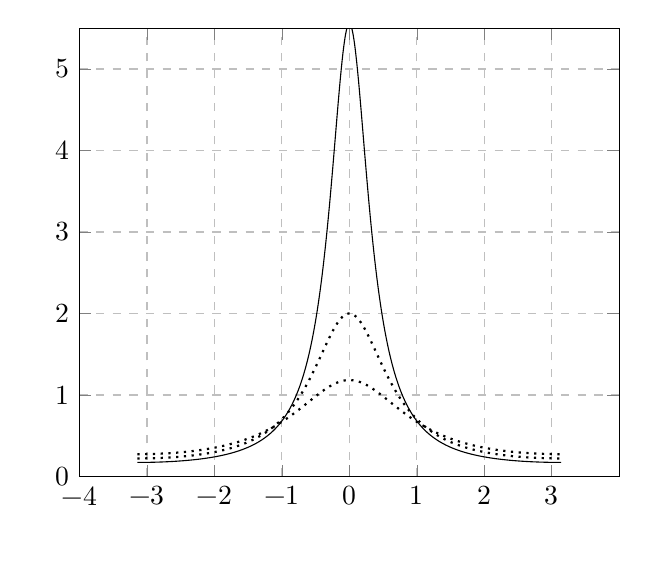
\begin{tikzpicture}[baseline]
                \begin{axis}[
                    xlabel={Ъглова честота},
                    ylabel={Амплитуда},
                    xmin=-4, xmax=4,
                    ymin=0, ymax=5.5,
                    xtick={-4, -3, -2, -1, 0, 1, 2, 3, 5.5},
                    ytick={0, 1, 2, 3, 4, 5, 6},
                    ymajorgrids=true,
                    xmajorgrids=true,
                    grid style=dashed,]
                    \addplot [domain=-pi:pi, samples=500,]{(1/(1 - 2*0.7*cos(deg(x)) + (0.7)^2))^1/2};
                    \addplot [domain=-pi:pi, samples=500, dotted, thick]{(1/(1 - 2*0.5*cos(deg(x)) + (0.5)^2))^1/2};
                    \addplot [domain=-pi:pi, samples=500, dotted, thick]{(1/(1 - 2*0.35*cos(deg(x)) + (0.35)^2))^1/2};
                    \end{axis}
            \end{tikzpicture}
            }\vfill
            \subfloat[Графика на $g(\omega)$ за различни стойност на $a$ и $b$]{%
            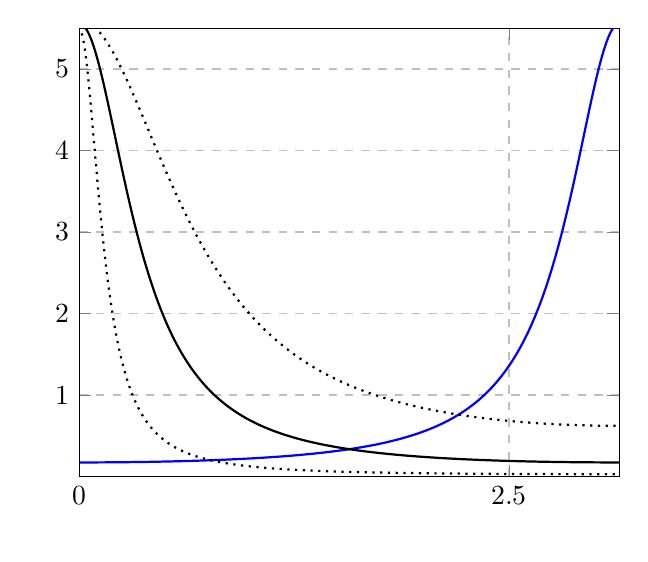
\begin{tikzpicture}[baseline]
                \begin{axis}[
                    xlabel={Ъглова честота},
                    ylabel={Амплитуда},
                    xmin=0, xmax=pi,
                    ymin=0, ymax=5.5,
                    xtick={0,2.5, 5},
                    ytick={1, 2, 3, 4, 5, 6},
                    ymajorgrids=true,
                    xmajorgrids=true,
                    grid style=dashed,]
                    \addplot [domain=-pi:pi, samples=500, thick, blue]{(1/(1 - 2*-0.7*cos(deg(x)) + (-0.7)^2))^1/2};
                    \addplot [domain=-pi:pi, samples=500, thick]{(1/(1 - 2*0.7*cos(deg(x)) + (0.7)^2))^1/2};
                    \addplot [domain=-pi:pi, samples=500, thick, dotted]{(2.8/(1 - 2*0.5*cos(deg(x)) + (0.5)^2))^1/2};
                    \addplot [domain=-pi:pi, samples=500, thick, dotted]{(0.2/(1 - 2*0.865*cos(deg(x)) + (0.865)^2))^1/2};
                \end{axis}
            \end{tikzpicture}
            }
            \caption{Действие IIR филтър от първи ред}
            \label{fig:appendix:2:2}
    \end{figure}   
    
    Понеже $a_1$ е реално число, винаги ще лежи на реалната ос, както е показано на полюс-нула графиката на $\autoref{fig:appendix:2:2}$
    
    Нека разгледаме $\mathcal{H}$ в честотния домейн:
    $\mathcal{H}(e^{\mathcal{i}\omega}) = \cfrac{b_0}{1 - a_1e^{-\mathcal{i}\omega}},$ където $\omega$ е ъглова честота, измерена в радиани.
    Можем изразим $\mathcal{H}$ като функция на $\omega$:

    \begin{flalign*}
        & \mathcal{H}(e^{\mathcal{i}\omega}) = \cfrac{b_0}{1 - a_1e^{-\mathcal{i}\omega}} = \cfrac{b_0}{1 - a_1 \cos{\omega} + \mathcal{i} a_1 \sin{\omega}} 
        = \cfrac{b_0(1 - a_1\cos{\omega} - \mathcal{i}a_1 \sin{\omega} )}{1 - 2 a_1 \cos{\omega} + a_1 ^ 2} && \\ 
        & = \frac{b_0(1 - a_1 \cos{\omega})}{{1 - 2 a_1 \cos{\omega} + a_1 ^ 2}} + \mathcal{i}\cfrac{- b_0 a_1 \sin{\omega}}{{1 - 2 a_1 \cos{\omega} + a_1 ^ 2}}&&
    \end{flalign*}
    Нека с $g(\omega)$ означим модула на $\mathcal{H}$
    \begin{flalign*}
        & g(\omega) = \cfrac{b_0^2(1 - 2 a_1 \cos{\omega} + a_1^2)}{(1 - 2 a_1 \cos{\omega} + a_1 ^ 2)^2} = \cfrac{b_0^2}{1 - 2 a_1 \cos{\omega} + a_1 ^ 2} &&
    \end{flalign*}
    На $\autoref{fig:appendix:2:2}$ се вижда графиката на $g(\omega)$ за различни стойности на $a_1$ и $b_0$
    Такива филтри се наричат \textbf{резонатори}, тъй като честотите във върха на графиката ще се усилят.
    Резонаторите се описват главно чрез своята \textbf{амплитуда} - височината на максимума, \textbf{честота} - къде е върхът върху честотната ос, 
    \textbf{честотна лента} - колко е широка графиката, което определя колко честоти ще се усилят.

    В случая на IIR филтътр от първи ред, амплитудата и честотаната лента се определят от $a_1$ и $b_0$,
    а върха на графиката винаги ще е в 0. Тоест, този вид филтри могат да усилват само честотите около 0.

    
    \chapter{Приложение към \nameref{chap:speech}}
    
    \begin{theorem}
    \label{appendix:2:01}
        $\mathcal{V}(\mathcal{z})$ за $N=2$
    \end{theorem}
    
    \begin{proof}[\unskip\nopunct]
        \begin{flalign}
            \tag{\ref{eq:tubes:22}}
            & \frac{1}{\mathcal{V}(\mathcal{z})} = \frac{U_G(\mathcal{z})}{U_L(\mathcal{z})}  = \mathcal{z}^{N/2}\left[
                \begin{array}{cc}
                    \cfrac{2}{1+r_G}, & -\cfrac{2r_G}{1 + r_G} \\
                \end{array}
                \right] \prod_{i=1}^{N} {\hat{Q}_i} \left[ \begin{array}{cc}
                    1 \\
                    0
                \end{array}\right] = &&
            \end{flalign}
            \begin{flalign*}
                & = \mathcal{z}\left[
                    \begin{array}{cc}
                        \cfrac{2}{1+r_G}, & -\cfrac{2r_G}{1 + r_G} \\
                    \end{array}
                    \right] {\hat{Q}_1}{\hat{Q}_2} \left[ \begin{array}{cc}
                        1 \\
                        0
                    \end{array}\right] = && \\
                & \\
                & = \mathcal{z}\left[
                    \begin{array}{cc}
                        \cfrac{2}{1+r_G}, & -\cfrac{2r_G}{1 + r_G} \\
                    \end{array}
                    \right]
                    \left[\begin{array}{cc}
                        \cfrac{1}{1 + r_1} & \cfrac{-r_1}{1 + r_1} \\
                        & \\
                        \cfrac{-r_1 \mathcal{z}^{-1}}{1 + r_1} & \cfrac{\mathcal{z}^{-1}}{1 + r_1} \\
                    \end{array}\right]
                    \left[\begin{array}{cc}
                        \cfrac{1}{1 + r_2} & \cfrac{-r_2}{1 + r_2} \\
                        & \\
                        \cfrac{-r_2 \mathcal{z}^{-1}}{1 + r_2} & \cfrac{\mathcal{z}^{-1}}{1 + r_2} \\
                    \end{array}\right]
                    \left[ \begin{array}{cc}
                        1 \\
                        0
                    \end{array}\right] = && \\
                &\\
                & = 2\mathcal{z}
                \left[
                    \begin{array}{cc}
                        \cfrac{1 + r_G r_1\mathcal{z}^{-1}}{(1+r_G)(1 + r_1)}, & -\cfrac{r_1 + r_G\mathcal{z}^{-1}}{(1 + r_G)(1 + r_1)} \\
                    \end{array}
                \right]
                \left[\begin{array}{cc}
                    \cfrac{1}{1 + r_2} & \cfrac{-r_2}{1 + r_2} \\
                    & \\
                    \cfrac{-r_2 \mathcal{z}^{-1}}{1 + r_2} & \cfrac{\mathcal{z}^{-1}}{1 + r_2} \\
                \end{array}\right]
                \left[ \begin{array}{cc}
                    1 \\
                    0
                \end{array}\right] = && \\
                &\\
                & = 2\mathcal{z}
                \left[
                    \begin{array}{cc}
                        \cfrac{1 + r_Gr_1\mathcal{z}^{-1} + r_1r_2\mathcal{z}^{-1} + r_Gr_2\mathcal{z}^{-2}}{(1+r_G)(1 + r_1)(1 + r_2)}, & -\cfrac{r_2 + r_Gr_1r_2\mathcal{z}^{-1} + r_1\mathcal{z}^{-1} + r_G\mathcal{z}^{-2}}{(1 + r_G)(1 + r_1)(1 + r_2)} \\
                    \end{array}
                \right]
                \left[ \begin{array}{cc}
                    1 \\
                    0
                \end{array}\right]&& \\
            \end{flalign*}
        \begin{flalign*}
            & \iff && \\
            & \mathcal{V}(\mathcal{z}) = \cfrac{0.5 (1+r_G)\prod\limits_{i=1}^{2}(1 + r_i)\mathcal{z}^{-1}}{1 + (r_Gr_1 + r_1r_2)\mathcal{z}^{-1} + (r_Gr_2)\mathcal{z}^{-2}} &&
        \end{flalign*}
        
        
        \end{proof}



\end{appendices}
        
\end{document}